\chapter{提案}
本章では,SBCを用いたマルチディスプレイシステムにおけるOS仮想化技術を用いた仮想化と,コンテナ技術を用いたSBCマルチディスプレイシステムのフレーム処理並列化を設計・提案する.
本章では,まず3.1節でOS仮想化基盤とコンテナ技術について簡単に説明する.
そして,続く3.2節でOS仮想化基盤を利用したSBCマルチディスプレイシステムのコンテナ仮想化についての設計と実装について述べる.
3.3章では映像ベースのアプリケーションをコンテナ仮想化することによって生じる問題と,その解決法について述べる.
3.4章では,本研究の中心部分となるヘッドノード内におけるフレーム処理の改良についての設計指針を述べ,具体的な実装について述べる.

\section{OS仮想化基盤とコンテナ技術}
OS仮想化基盤には,代表的なものとしてDocker \cite{docker,using_docker}がある.
Dockerは,Docker社が開発しているプラットフォームであり,Dockerを用いることでマシン内にコンテナと呼ばれる仮想環境を作成し,実行することができる.

DockerをはじめとしたOS仮想化と比較されるのが,ハイパーバイザ型仮想化である.
ハイパーバイザ型仮想化は,ホストマシンとなる物理マシン上でハイパーバイザと呼ばれる仮想マシン (VM) を作成および実行するソフトウェアを動作させ,それを通じて仮想化環境を制御するものである.
ハイパーバイザ型仮想化は,移植面で汎用性が高いことが長所である.
一方で,ホストOSを介して仮想環境の制御を行うため,制御のオーバーヘッドが大きく処理が低速になるという欠点を持つ.
それに対して,コンテナを用いたOS仮想化技術では仮想化環境 (コンテナ) はホストマシンのOSを使用する.
そのためコンテナは軽量に動作させることが可能であり,仮想環境の起動や終了も小さいオーバーヘッドで行えることが特徴である.

コンテナ技術を用いたOS仮想化とハイパーバイザ型仮想化の概要を図\ref{docker}に示す.

\begin{figure}[H]
    \hspace*{\fill}
    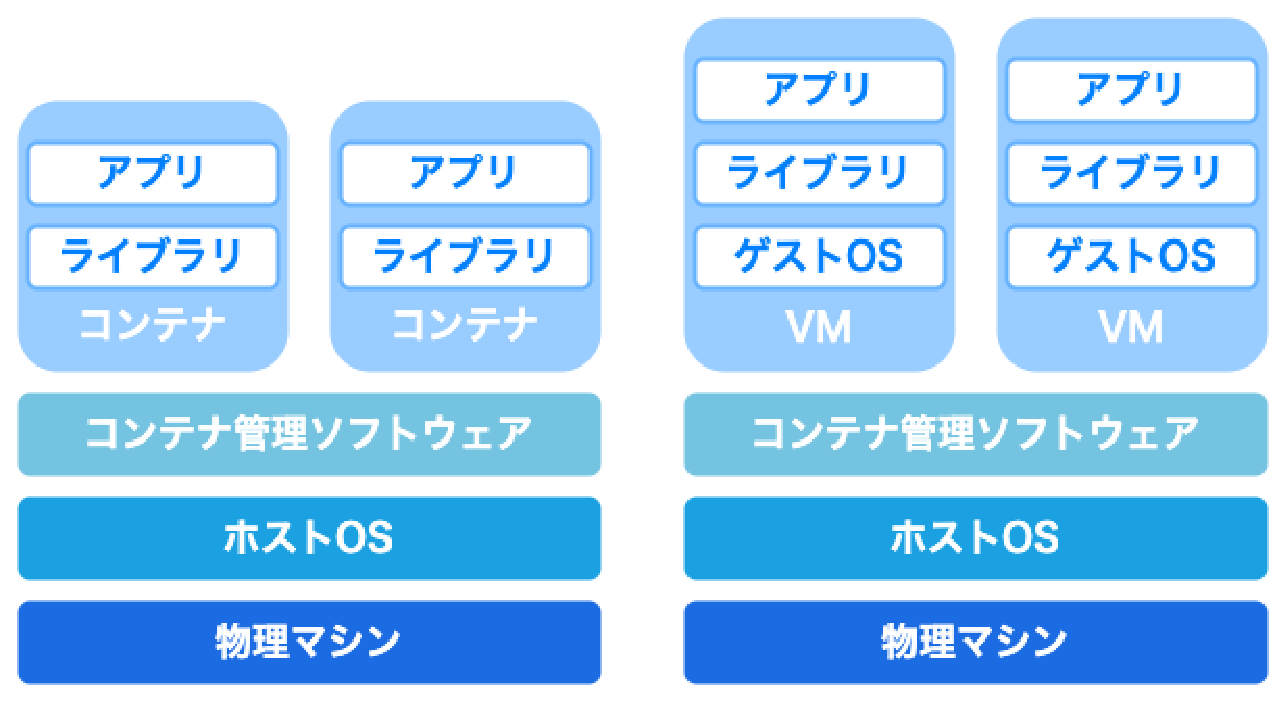
\includegraphics[width=\linewidth]{./fig/chap3/docker.eps}
    \hspace*{\fill}
    \caption{コンテナ技術を用いたOS仮想化とハイパーバイザ型仮想化}
    \label{docker}
\end{figure}

さらに,Dockerを利用することでさまざまな利点も生まれる.

まず,仮想化環境をコード化して管理する事で,どのような環境の上にでも同一の環境を作成する事ができるという点である.
Dockerでは仮想化環境の構築情報をコード化されたファイルとして管理する.
このファイルを保存し配布する事で特定の環境を再現し,複数のマシン上で全く同一の環境を作り出すことが可能となる.
この機能は,ソフトウェアの開発やテストなどで異なるマシンに同一の環境を作成し,その上でアプリケーションを動作させる必要のある場合などによく利用されている.

また,環境の作成や廃棄が簡単であることも利点の1つである.
複数のサーバを連携させて全体で1台のサーバであるかのように動作させるクラスタシステムを構築する場合も,Dockerイメージがあればそれを元に複数の環境(コンテナ)を起動できる.
この機能を活用することにより開発環境,動作環境をはじめから作る必要がなくなり,クラスタシステムを構築することも容易になる.
さらに,Kubernetes \cite{k8s}などが有するコンテナオーケストレーションシステムを用いてクラスタ環境を管理することもできる.

\section{マルチディスプレイシステムのコンテナ化}
前節で紹介したような仮想化技術を用いることで,異なるマシンでもアプリケーションを同一の環境で動作させることができる.
この仮想化技術を用いて,2章で先行研究として紹介したSBCを用いたマルチディスプレイシステムの仮想化を検討する.

先行研究では,SBCマルチディスプレイシステムにおいてディスプレイノードとしてRaspberry Piを使用している.
2022年2月現在においてはSBCの開発が盛んに行われており,市場には数百種類ものSBCが存在している \cite{hackerbords}.
それらのSBCの間ではアーキテクチャ,OS,ディスプレイの描画方法,対応言語などに違いが存在する.
そのため,これらのSBCを用いてマルチディスプレイを構築する場合には構築の手順や動作に異なる点が生じることが予想される.
異なるSBCを用いた際に発生するこれらの差異を吸収するためには,さまざまなSBCに対応することができるマルチディスプレイ構築用ミドルウェアの開発が必要である.
そこで,前節で紹介したコンテナ仮想化技術であるDockerの利用を検討する.

\begin{figure}[H]
    \hspace*{\fill}
    \includegraphics[width=\linewidth]{./fig/chap3/md_docker.eps}
    \hspace*{\fill}
    \caption{Dockerを用いた環境構築}
    \label{docker_usage}
\end{figure}

Dockerを用いた環境構築の概要図を図\ref{docker_usage}に示す.
ユーザは,まずヘッドノードもしくはディスプレイノードとして利用するマシンに対してDockerのインストールを行う.
次に, Dockerに用意されているコマンドを用いてGitHub \cite{github}上のリポジトリからソースコードを取得し,その中に含まれているDockerfileを用いてホストマシン内にコンテナ環境を作成する.
ここでDockerfileとはコンテナ環境の構成情報 (OS,パッケージ,ネットワーク設定情報など) を保存したファイルであり,これを用いてコンテナ環境を構築することによりファイルによってあらかじめ設定されていた環境を簡単に構築することができる.
最後にホストマシン上に構成したコンテナ環境内でプログラムのビルドを行う事で,そのマシンをヘッドノードもしくはディスプレイノードとして使用することが可能になる.

\section{コンテナ環境におけるディスプレイの制御}
本節では,コンテナ技術を用いて構築したMDにおけるフレーム表示時に生じる問題とその対処について説明する.
マシンに接続されたディスプレイに画像フレームを表示する際には,一般にフレームバッファとよばれる領域が使用される.
フレームバッファはマシンの/devディレクトリに存在するデバイスファイルである.
このファイルの中にディスプレイに表示するデータを格納することで,OSがディスプレイに画像を描画するという仕組みになっている.
フレームバッファを用いたディスプレイへの画像表示の概要を図\ref{framebuffer}に示す.

\begin{figure}[H]
    \hspace*{\fill}
    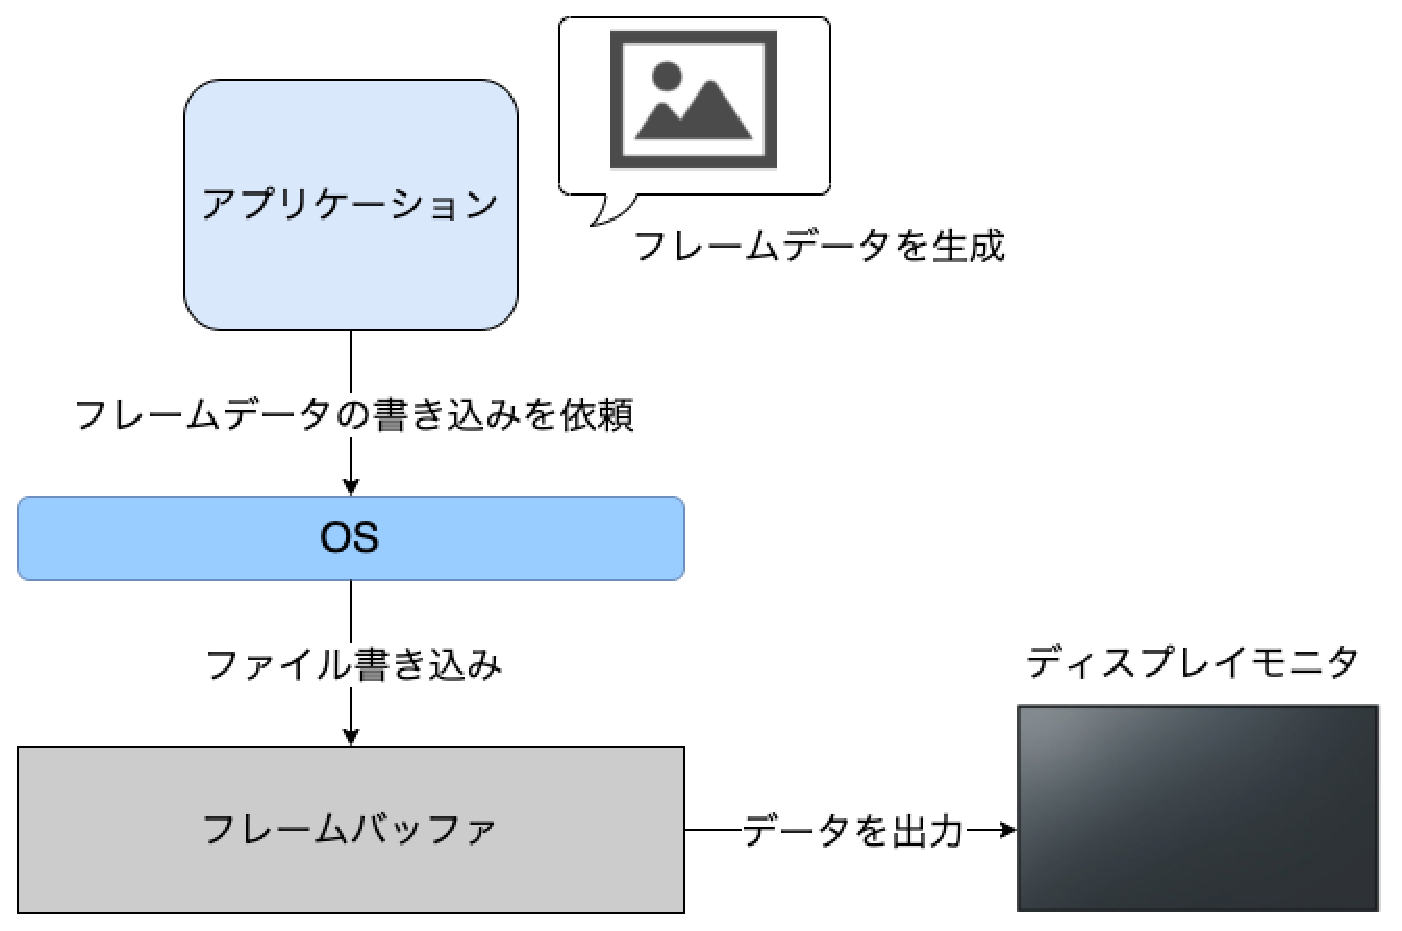
\includegraphics[width=\linewidth]{./fig/chap3/framebuffer.eps}
    \hspace*{\fill}
    \caption{フレームバッファを用いたディスプレイ表示}
    \label{framebuffer}
\end{figure}

Dockerを用いて構築したコンテナ環境の内部からは,ホストマシンのリソースへのアクセスが制限される場合がある.
例えば,デフォルトの状態ではDockerコンテナはDockerコンテナの内部でDockerデーモンの起動を行うことができない.
これは、デフォルトではコンテナからホストマシンのデバイスへのアクセスが許されていないことが原因である.
同様に,フレームバッファもDockerコンテナの内部から見ればホストマシン内のデバイスファイルであるため,ファイルが操作できずに画像フレームデータをディスプレイへの表示することができなくなっている.
この状態を,コンテナはunprivilegedな状態であるという.

対して,privilegedなコンテナはホストマシンの全てのリソースにアクセスする事ができる.
コンテナをpriviledgeな状態で起動するためには,起動時のコマンドで--privilegedコマンドを指定する必要がある.

\section{ヘッドノードでのフレーム処理の改良}
ここまでに紹介した技術を用いることで,SBCマルチディスプレイシステムをコンテナ基盤上で動作させることができるようになる.
続いて本節以降では,本研究の提案の中心部分となるヘッドノードでのフレーム処理の改良について述べる.

2章でも説明した通り,先行研究で提案されたマルチディスプレイには高解像度な動画や高フレームレートな動画をMD上に表示しようとするとヘッドノードでの処理がボトルネックとなり,動画表示に遅延が発生するという問題点がある.
高解像度な動画はフレームの分割や圧縮にかかる時間が大きくなるためヘッドノード内での処理時間が増加し,フレームの表示処理への影響も大きくなる.
また,高フレームレートな動画の場合にはフレーム処理時間の影響により元々のフレームレートを維持したまま動画を表示することが困難になる.
さらに,大規模なMDを構築した際のパフォーマンス低下も問題点としてあげられる.
先行研究のMDではヘッドノード内でフレーム圧縮を行うスレッドが1つであるため,MDを構成するディスプレイ数が増加するのに伴ってスレッドでの処理負荷が増加する.
その結果,MDの大規模化に伴ってフレーム処理にかかる時間も増加し,動画再生時のフレームレートが低下する.

この問題に対して,提案手法ではヘッドノードでのフレーム処理を並列化したプロセスとして実装し,ヘッドノード内でのフレーム処理時間の短縮を目指す.

\subsection*{フレーム処理のコンテナ並列化}
提案手法の実装にはOS仮想化技術を用いたコンテナ技術を使用し,プロセスレベルでの処理並列化を図る.
また,処理の並列化に伴うプロセス間での画像フレームの受け渡しについては,高速なプロセス間通信が可能な共有メモリを使用することでオーバーヘッドの低減を目指す.

先行研究では,ヘッドノード内の圧縮スレッド内でフレーム切り出し,フレーム分割,フレーム圧縮の3種類の処理が行われている.
フレーム切り出しとフレーム分割はディスプレイ数に関わらず1フレームに対して1回の処理のみが行われる.
しかし一方で,フレームの圧縮はマルチディスプレイを構成するディスプレイ数に応じて処理回数が変化する.
そのため,構成ディスプレイを増加させた場合にはこの部分がシステムのボトルネックとなる.
このボトルネックを解消するために,圧縮処理をヘッドノード内で並列化して行い,全体でのフレーム処理時間の短縮を試みる.

\begin{figure}[H]
    \hspace*{\fill}
    \includegraphics[width=\linewidth]{./fig/chap3/process_parallelization.eps}
    \hspace*{\fill}
    \caption{フレーム処理の並列化}
    \label{process_para}
\end{figure}

図\ref{process_para}に,提案手法におけるヘッドノード内のコンテナ構成を示す.
提案手法ではヘッドノード内で行われる処理それぞれを単一のコンテナに分割し,画像フレームの切り出し・分割を行う分割コンテナ,フレームの圧縮処理を行う圧縮コンテナ,そしてディスプレイノードとの同期用通信を行う同期制御コンテナの3種類のコンテナとして実装する.
圧縮コンテナは構成ディスプレイと同じ数だけ用意し,ヘッドノード内で並列化してフレームの圧縮処理を行う.

\subsection*{コンテナ間でのフレーム受け渡し処理}

処理の並列化を目的としてフレームの分割を行うコンテナと圧縮を行うコンテナを分けたことにより,ヘッドノード内のコンテナ間で画像フレームの受け渡しを行う必要が生じる.
この処理によるオーバヘッドを抑えるために,高速なプロセス通信が可能な共有メモリ (System V IPC) \cite{kerrisk2010linux,linux_kernel}を使用する.

以下,共有メモリ (System V IPC) について簡単に説明する.
IPCとはプロセス間通信 (InterProcess Communication) の略であり,ユーザモードプロセスから

\begin{itemize}
    \item セマフォを利用した他のプロセスとの同期
    \item 他のプロセスとの間でのメッセージ送受信
    \item 他のプロセスとのメモリ領域の共有
\end{itemize}

などの操作を行う事ができる.

System V IPCは,現在ではLinuxを含むほとんどのUNIXシステムで使用できるようになっている.
IPCのデータ構造は,プロセスがIPC資源 (セマフォ,メッセージキュー,共有メモリリージョン) を要求した際に動的に作成される.
IPC資源を要求したプロセスが獲得した資源を明示的に解放しない限りIPC資源はメモリ上に残り続け,他のどのプロセスからでも使用できる状態になる.
各資源は,ファイルシステムツリーにおけるファイルのパス名に相当する32ビットのIPCキーによって識別される.
また,各IPC資源は32ビットのIPC識別子を持つ.
IPC資源はカーネルによって決定されるが,IPCキーは自由に決める事が可能である.
複数のプロセスがIPC資源を利用する際には,IPC識別子が利用される.
本研究の実装ではSystem V IPCを利用して共有メモリ領域を獲得し,異なるプロセス間でのデータ共有を高速に行うことを目的とする.

続いて,IPC資源の利用方法について説明する.
System V IPCを用いて共有メモリ領域を獲得するためには,shmget()関数を使用する.
shmget()関数は引数として渡されたIPCに対応するIPC識別子を取得し,そのIPC識別子を利用することでプロセスが共有メモリ領域にアクセスすることができるようになる.
別々のプロセスから同一のIPC資源を共有するための方法は2通り存在する.
1つはプロセス間であらかじめ固定のIPCキーを決定しておく方法である.
この方法は単純であるため,多くのプロセスが関連する複雑なアプリケーションで利用してもうまく動作する.
しかし,全く関係ないプロセスが偶然同じIPCキーを使用してしまう可能性がある.
もう1つは,一方のプロセスでIPCキーにIPC\_PRIVATEを指定する方法である.
この方法では新規のIPC資源が割り当てられ, そのIPC識別子によってアプリケーション内の他のプロセスとの通信を行うため,他のプロセスから誤ってIPC資源を利用されてしまうことを防げる.

以上の方式を検討した結果,本研究では複数のコンテナ間でのデータの受け渡し処理に使用することを想定しており,IPC資源が複数のプロセスから参照されることになるため,実装が容易になる前者の手法を採用した.

\subsection*{IPC共有メモリ}

IPC共有メモリでは,共有するデータ構造をIPC共有メモリリージョンに配置することにより,複数のプロセスから共有データ構造にアクセスする事ができる.
以下,IPC共有メモリの使用方法について述べる.
プロセス1とプロセス2の2つの異なるプロセスの間で共有メモリ領域を作成するメモリ領域を作成するとする.
まずプロセス1はプロセス2との間で一意となるIPCキーを作成する.
そして,このキーを用いてshmget()関数によりIPC識別子を取得する.
この時に,獲得する共有メモリ領域のサイズやパーミッションなどを決める事ができる.
続いて,IPC識別子を引数としてshmat()関数を実行することにより,共有メモリがプロセス1のメモリ領域にアタッチされ,プロセス1から共有メモリ領域へのアクセスが可能になる.

もう一方のプロセス2では,プロセス1が生成したIPCキーを取得する.
続いてプロセス1と同様に取得したIPCキーを引数としてshmget()関数を実行し,共有メモリのIPC識別子を取得する.
その後,IPC識別子を引数としてshmat()関数を実行して共有メモリをプロセス2のアドレス空間にアタッチすることでプロセス2からもプロセス1と同じ共有メモリ領域を使用することができるようになる.
以上に述べたような一連の手続きを行うことで,作成した共有メモリ領域を利用して異なるプロセスとの間でデータを共有することが可能になる (図\ref{shared_memory}).

\begin{figure}[H]
    \hspace*{\fill}
    \includegraphics[width=\linewidth]{./fig/chap3/ipc1.eps}
    \hspace*{\fill}
    
\end{figure}

\begin{figure}[H]
    \hspace*{\fill}
    \includegraphics[width=\linewidth]{./fig/chap3/ipc2.eps}
    \hspace*{\fill}
\end{figure}


\begin{figure}[H]
    \hspace*{\fill}
    \includegraphics[width=\linewidth]{./fig/chap3/ipc3.eps}
    \hspace*{\fill}
\end{figure}

\begin{figure}[H]
    \hspace*{\fill}
    \includegraphics[width=\linewidth]{./fig/chap3/ipc4.eps}
    \hspace*{\fill}
    \caption{共有メモリ使用の流れ}
    \label{shared_memory}
\end{figure}

\subsection*{フレーム受け渡し機能の実装}

続いて,フレーム受け渡し機能の具体的な実装について説明する.
共有メモリは,ヘッドノード内で動作する分割コンテナと圧縮コンテナとの間で画像フレームデータを共有するために利用する.
分割コンテナは,動画ファイルから画像フレームの切り出し処理を行う.
このとき,画像処理にはオープンソースのコンピュータビジョンライブラリであるOpenCVを使用する.
OpenCVにおいて画像フレームはMatという型で管理される.
Mat型は画像フレームに関するパラメータを持った構造体であり,画像フレームの縦横ピクセル数,画像フレームの色深度,画像フレームのデータへのポインタなどをメンバとして保持している.
Mat構造体の内容を図\ref{mat}に示す.

\begin{figure}[H]
    \hspace*{\fill}
    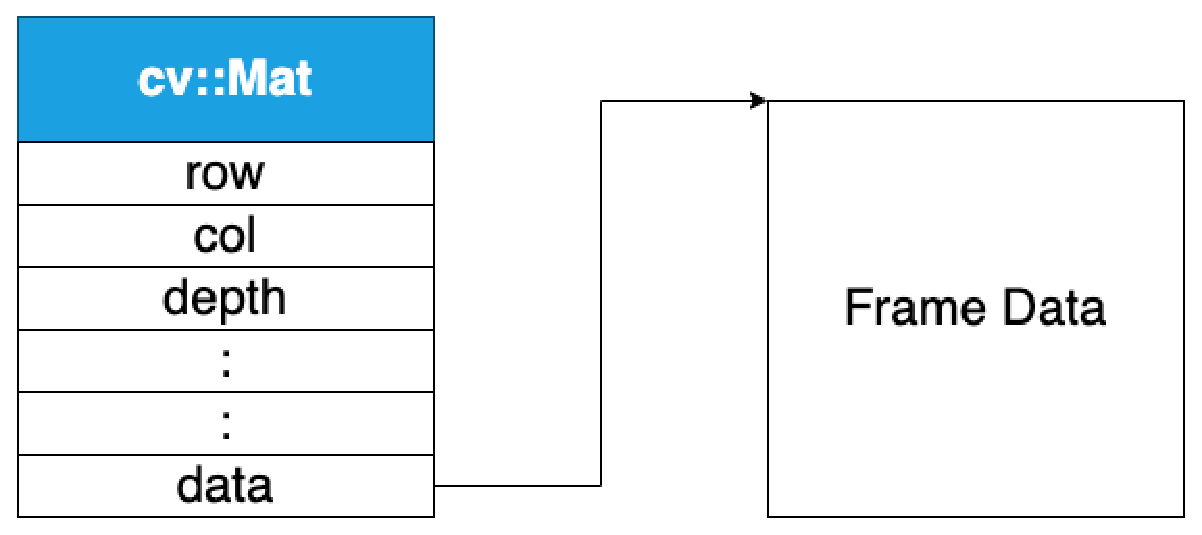
\includegraphics[width=120mm]{./fig/chap3/mat.eps}
    \hspace*{\fill}
    \caption{OpenCVにおけるMat構造体}
    \label{mat}
\end{figure}

プロセス間でのフレームデータ共有を行うためには,このMat型の構造体を共有メモリに格納し,プロセス間で共有できるようにすることが必要である.
しかし,Mat型の構造体を単純な操作で共有メモリに格納するだけではフレームデータそのものの受け渡しは実現できない.
これはMat構造体はフレームデータの実態ではなくデータ格納場所を指すポインタのみを保持しており,フレーム切り出しの際に画像フレームの画素データ本体が格納されるのはそのプロセスに固有のメモリ空間であるためである.
そこで本実装では,分割コンテナと圧縮コンテナとの間に作成した共有メモリ領域をchar型の配列として定義し,Mat構造体のもつフレームデータ格納場所へのポインタの値を利用してmemcpy()関数によるコピーを行っている.
memcpy()関数は引数を3つ持ち,引数1を先頭としたメモリ領域に,引数2を先頭としたメモリから引数3バイト分のデータをコピーする.
memcpy()関数によるメモリのコピーは非常に高速に動作するため,共有メモリ領域への書き込みで生じるオーバーヘッドは小さくなる.

実際の処理では,まず分割コンテナがフレームの切り出しと分割を行った後,圧縮コンテナとの間に作成された共有メモリにフレームデータを格納する.
圧縮コンテナは共有メモリに格納されたフレームを取得し,圧縮処理を行う.

共有メモリはヘッドノードの中に1つのみを作成し,その中でそれぞれの圧縮コンテナに対してメモリ領域を分割して割り当てるという手法を採用する.
また,共有メモリにはフレーム切り出しの際に使われるOpenCVのMat形式を文字型の配列に変換してからフレームデータを格納する(図\ref{shared_memory2}).

\begin{figure}[H]
    \hspace*{\fill}
    \includegraphics[width=\linewidth]{./fig/chap3/shared_memory2.eps}
    \hspace*{\fill}
    \caption{共有メモリの使用例}
    \label{shared_memory2}
\end{figure}

\subsection*{フレーム受け渡し処理の詳細}

続いて,共有メモリ領域を用いたフレームデータの受け渡しについて詳細な動作を説明する.
フレームデータ受け渡しに用いる共有メモリ領域は,はじめに分割ノードによってホストマシン内に1つだけ作成される.
その1つの共有メモリ領域に対して分割メモリはフレームデータの格納を行う.
接続ディスプレイと同数だけ用意された全ての圧縮コンテナは1つの共有メモリに対してデータの取り出しを行う.
また,作成したメモリの共有を行うには共有メモリを作成した際に使用されたIPCキーを分割ノードと圧縮ノードとの間で共有する事が必要になる.
このIPCキーの共有にはホストマシンのメモリ領域を利用している.
まず,分割ノードにより共有メモリの作成に使用されたIPCはあらかじめ設定されたパスに存在する物理マシン内のテキストファイルに文字列として保存される.
その後起動された圧縮コンテナが物理マシン内の該当パスに存在するフォルダを認識し,その中に記述されているIPCキーを引数としてコンテナ内でプログラムを実行する.
この仕組みによって分割コンテナと圧縮コンテナとの間でIPCキーを共有することができ,同一のメモリ領域にアクセスする事が可能になる(図\ref{key_share}).

\begin{figure}[H]
    \hspace*{\fill}
    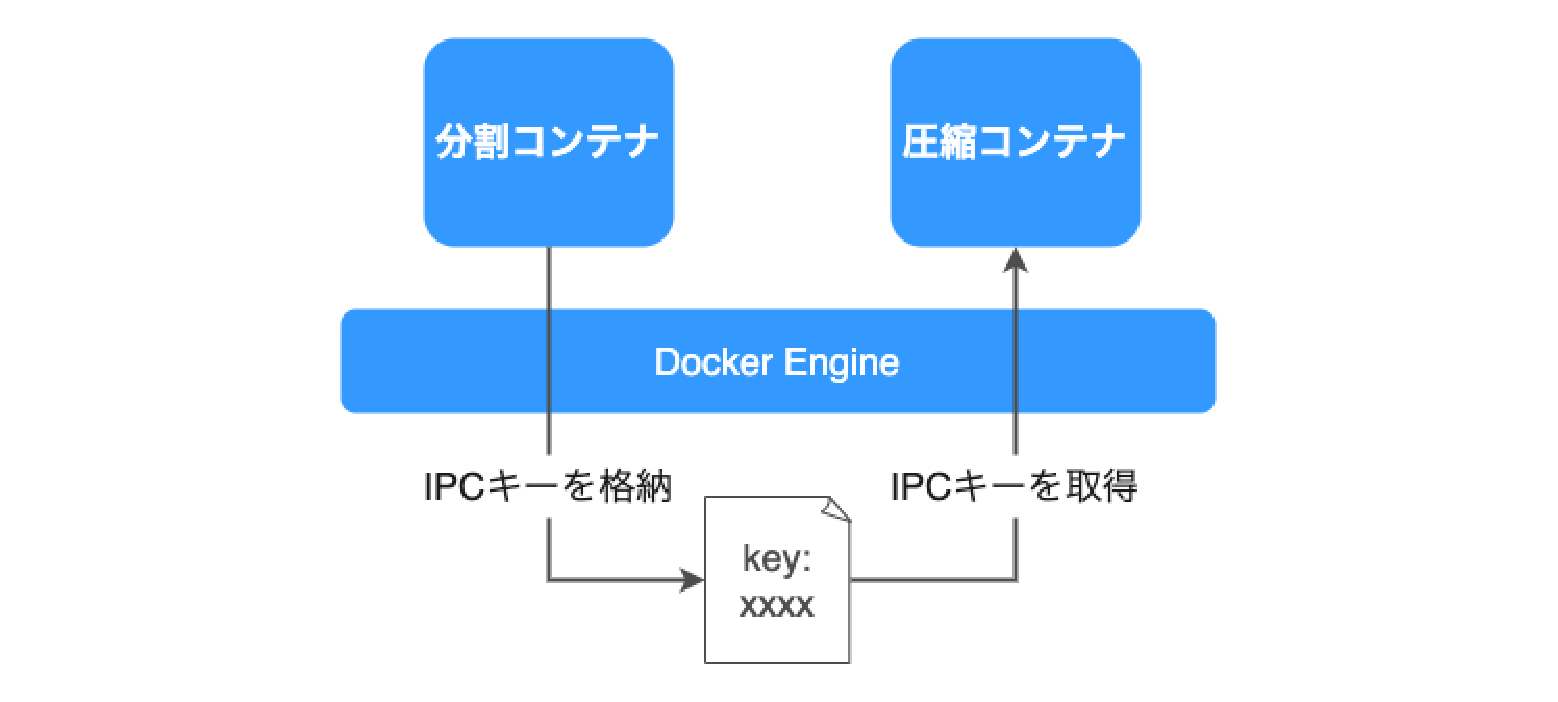
\includegraphics[width=\linewidth]{./fig/chap3/ipckeyshare.eps}
    \hspace*{\fill}
    \caption{プロセス間でのIPCキー共有}
    \label{key_share}
\end{figure}

共有メモリ領域では,フレームの格納および取り出しを高速で行うために,分割コンテナによって格納された分割済みの画像フレームデータをバッファリングする仕組みを用意する.
共有メモリに格納される画像フレームデータは,ディスプレイノードが接続しているディスプレイと同じ解像度となる.
本研究では,動画の表示に使用されるディスプレイモニタの解像度としてFull HD (1920 x 1080ピクセル) のものを想定する.
また,色深度は赤,緑,青の3深度とする.
この想定下では,共有メモリに格納される分割後の画像フレームは1920 x 1080ピクセル,色深度3, ビット深度 (1ピクセル,1色のデータを保持するのに必要なビット数)8となり,そのデータ量はおよそ5.9MBとなる.
よって,各圧縮コンテナに対して8枚の分割済みフレームをバッファリングするとすると,必要な共有メモリの領域は(圧縮コンテナ数) x 5.9 x 8 (MB) で算出することができる.
例えば,4面構成のマルチディスプレイを構築する場合には約189MB, 9面構成のマルチディスプレイを構築する場合には約425MBの共有メモリ領域が必要となる.
このメモリ領域を,分割コンテナは起動と同時に獲得する処理を行う.

分割コンテナは,新たなフレームの切り出しを行いそれに対する分割処理を完了すると,共有メモリ領域に用意されたバッファに順次フレームを格納していく.
バッファにはそれぞれの圧縮コンテナに対して領域を定めておき,圧縮コンテナはその領域から順番にフレームの取り出しを行い後続の処理を開始する.
共有メモリ領域に作成されたバッファを用いてコンテナ間で画像フレームの受け渡しを行う様子を,図\ref{buffer}に示す.

\begin{figure}[H]
    \hspace*{\fill}
    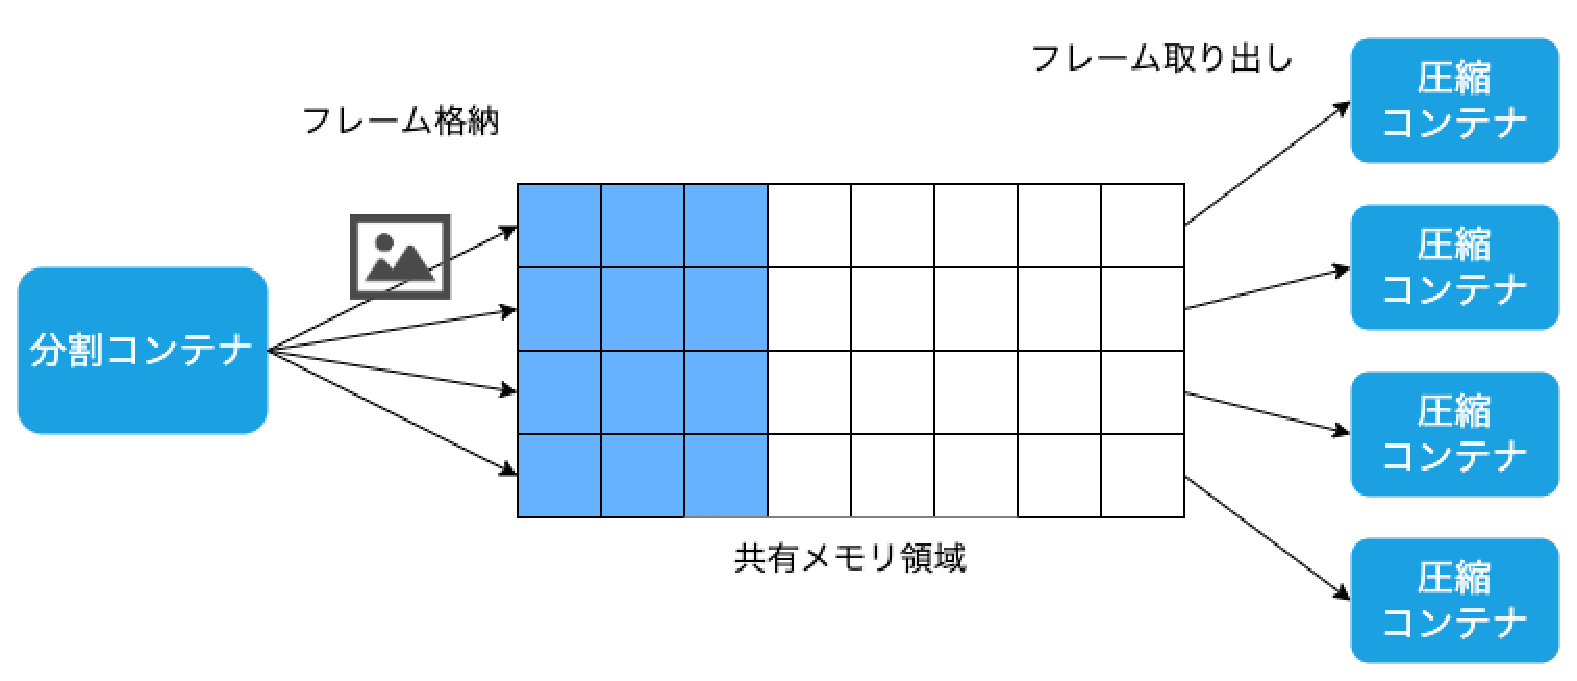
\includegraphics[width=\linewidth]{./fig/chap3/buffering.eps}
    \hspace*{\fill}
    \caption{共有メモリ内におけるフレームのバッファリング}
    \label{buffer}
\end{figure}

\subsection*{各コンテナでの処理}
ここでは,各コンテナ内での処理について順に述べる,
図\ref{divide_container}および図\ref{compress_container}に提案手法における分割コンテナと圧縮コンテナの処理フローチャートを示す.

\begin{figure}[H]
    \hspace*{\fill}
    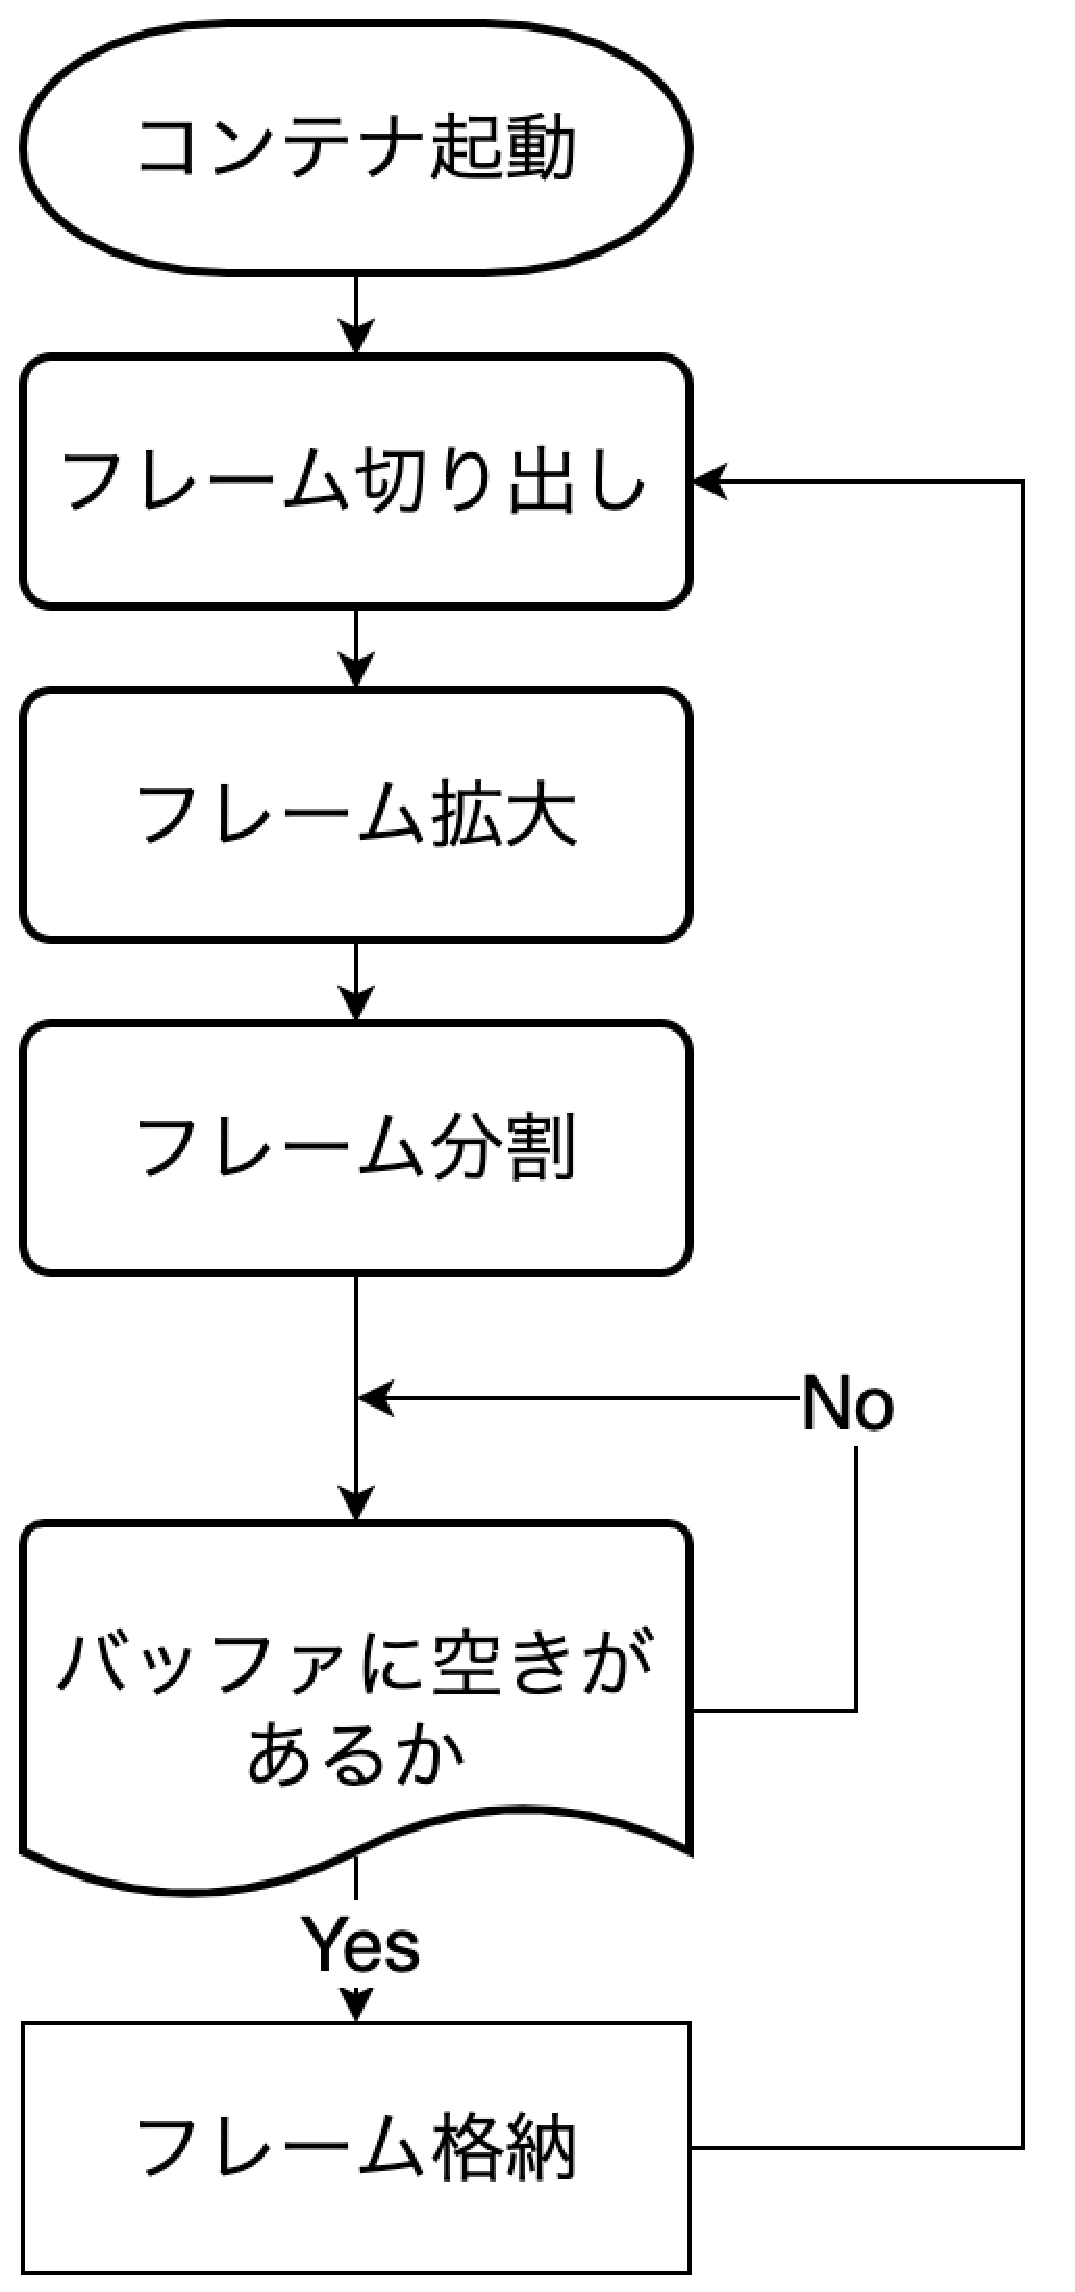
\includegraphics[width=50mm]{./fig/chap3/bunkatu_flow.eps}
    \hspace*{\fill}
    \caption{分割コンテナの動作フロー}
    \label{divide_container}
\end{figure}

分割コンテナは,コンテナが起動されるとすぐに動画ファイルからのフレーム切り出し処理を開始する.
その後,切り出したフレームに対して,構築したマルチディスプレイの解像度に応じたサイズにフレームの拡大処理を行う.
次に,ディスプレイの数に応じた分割処理を行い,共有メモリに作成されたバッファに順に格納していく.
このとき,共有メモリ内のバッファにはあらかじめ用意したバッファの数以上のフレームを格納する事ができない.
そのため,フレームの格納処理を行う前にバッファに格納されているフレーム数を取得し,バッファ上にあるフレーム数が上限に達していれば格納処理を行わずに待機状態になる.
その後,圧縮フレームがバッファから画像フレームを取り出すことによってバッファに空きができたことを認識すると待機状態を終了し,現在処理中のフレームデータを格納して次のフレームの処理へと移る.

\begin{figure}[H]
    \hspace*{\fill}
    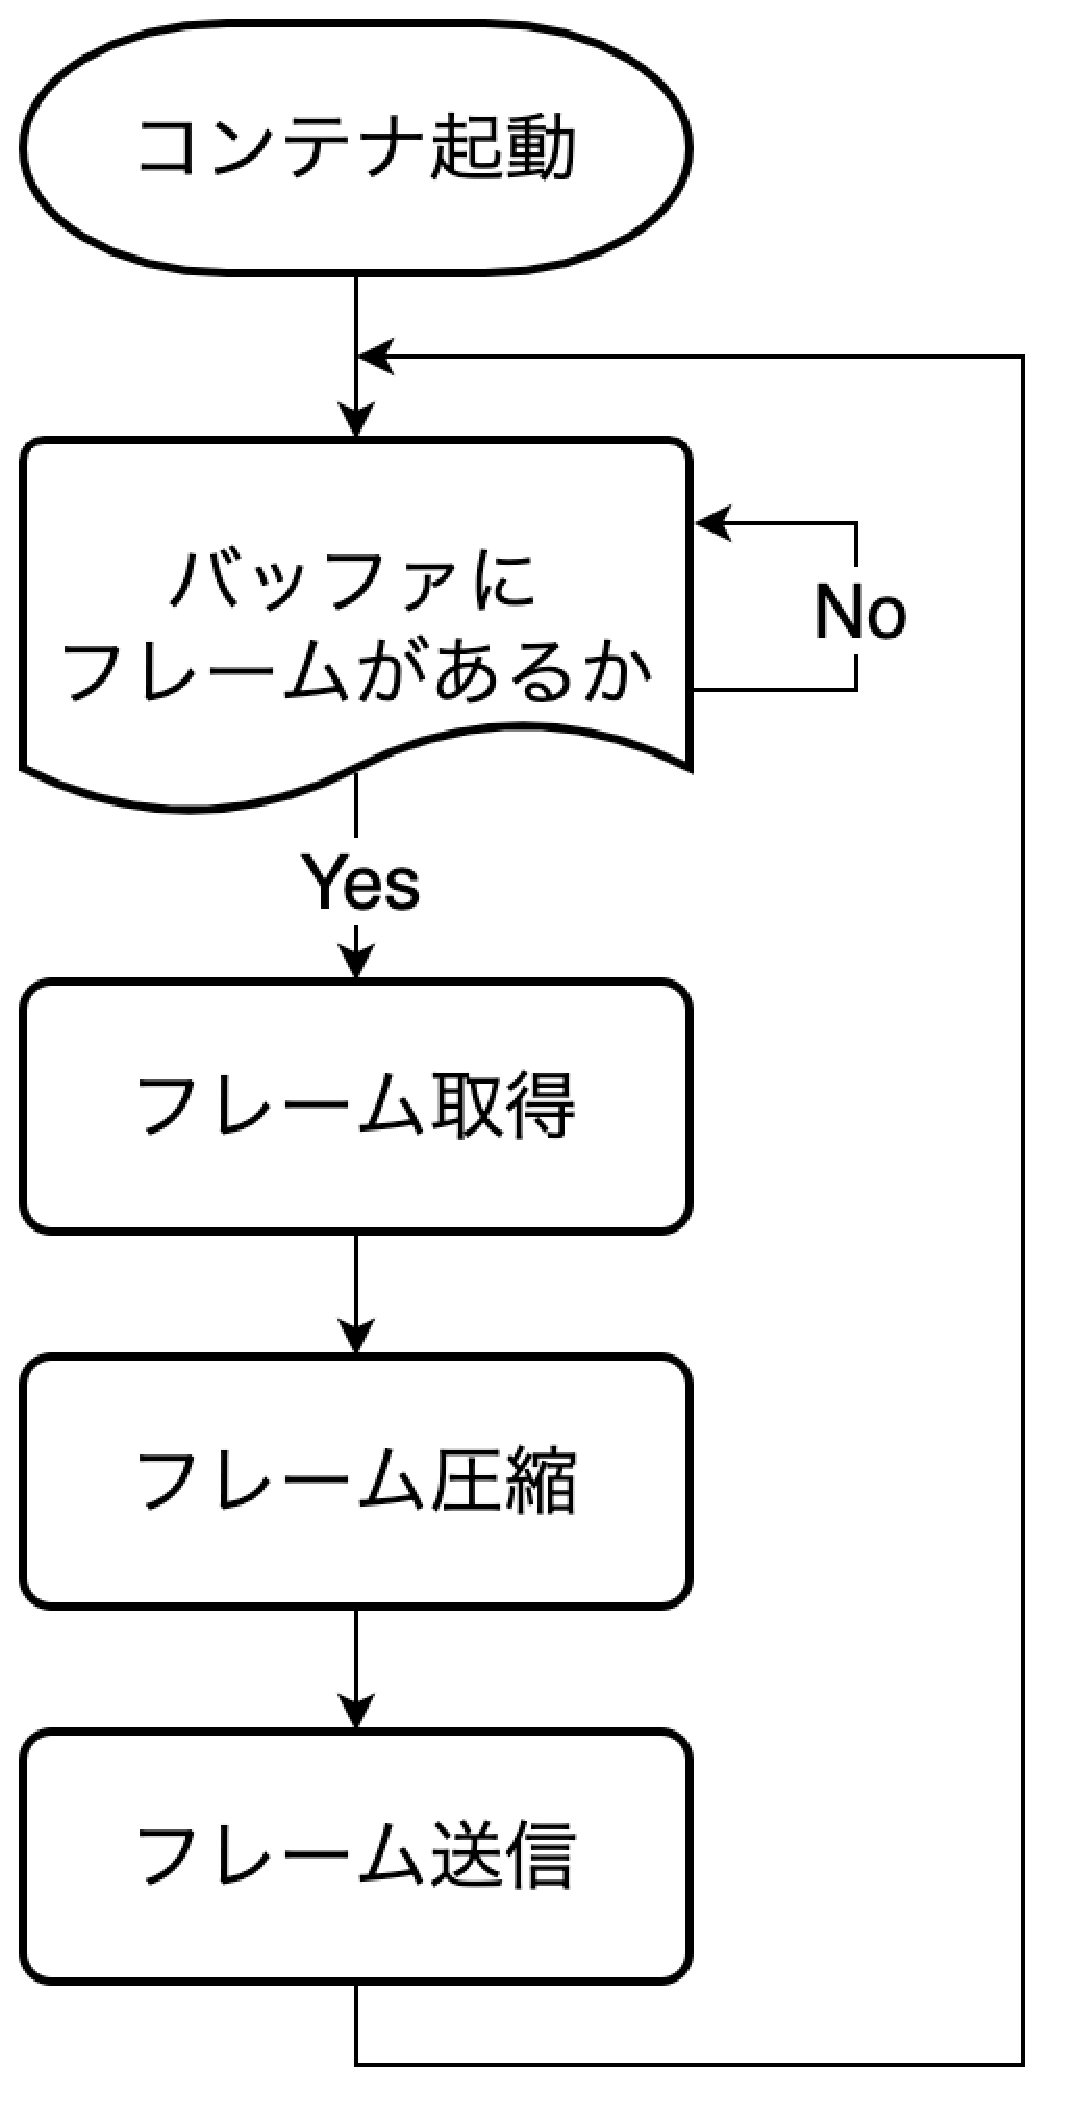
\includegraphics[width=50mm]{./fig/chap3/assyuku_flow.eps}
    \hspace*{\fill}
    \caption{圧縮コンテナの動作フロー}
    \label{compress_container}
\end{figure}

圧縮コンテナは起動と同時に分割コンテナとの共有メモリを取得し,バッファにフレームが格納されているかどうかの監視を開始する.
分割コンテナによってバッファに分割済みの画像フレームが格納されたことを確認すると監視を終了し,フレーム処理を開始する.
圧縮コンテナで行われるフレーム処理は,フレームの圧縮と送信である.
バッファから画像フレームを取り出して圧縮処理を行うと,OpenCVのMat形式から文字列オブジェクト (C++のstring型) への変換が行われる.
この文字列オブジェクトを接続したディスプレイノードへと送信するまでが各フレームに対する一連の処理となる.

\subsection*{提案手法を用いたマルチディスプレイシステムの構築}
最後に,提案手法を用いて構築したマルチディスプレイの全体像について述べる.
図\ref{system_flow_teian}に提案手法を用いて構築したMDの動作フローを示す.
ヘッドノードでは分割コンテナ,圧縮コンテナ,同期制御コンテナの3種類のコンテナが動作している.
処理の流れとしては,まず分割コンテナが動画ファイルから1フレームずつ切り出し,構成ディスプレイ数に応じて分割処理が行われた後,作成した共有メモリ領域に格納する.
圧縮コンテナは,共有メモリから分割済みの画像フレームを取得する.
圧縮コンテナはこのフレームに対してJPEG圧縮処理を行い,それぞれが接続しているディスプレイノードへの送信処理を行う.
圧縮コンテナからフレームを受け取ったディスプレイノードではフレーム展開処理を行い,展開後の画像フレームをホストマシンのフレームバッファに書き込むことでディスプレイへ画像を表示する.
この処理を各フレームに対して行うことで接続されたディスプレイ上への動画の再生が実現される.
また,ヘッドノードの内部では分割コンテナと複数の圧縮コンテナの他に同期制御コンテナも動作する.
同期制御コンテナの役割はディスプレイノードで動作している表示制御スレッドにフレームの表示命令を送信することである.
同期制御スレッドはディスプレイノードから各画像フレームが表示バッファに格納され,ディスプレイの表示準備が完了した旨の通知を受け取る.
この通知が全てのディスプレイノードから送信されたことを確認し,同期制御スレッドが各ディスプレイノードに対してフレームの表示命令を送信する.
さらに,同期制御スレッドは圧縮コンテナ内で行われているフレーム圧縮のパラメータを制御することでフレームレートを一定に保つ役割を持つ.


\begin{figure}[H]
    \hspace*{\fill}
    \includegraphics[width=\linewidth]{./fig/chap3/resume_fig1.eps}
    \hspace*{\fill}
    \caption{提案手法を用いたMDの動作フロー}
    \label{system_flow_teian}
\end{figure}
